% !TEX root = main.tex

\subsection*{Participants}
A convenience sample (N=9, 6 males, 3 females) was recruited via student mailing lists at the University of Helsinki. The participants were between 22-38 years of age (mean 27, SD 3) with normal or corrected-to-normal visual acuity and no history of neurological or psychiatric disease.

\begin{table}[ht]
\centering
\caption{\label{tab:Participants}Participant background information.}
\begin{tabular}{llllll}
\hline
Participant & Gender & Age & Driving license & Driving experience (km) & Gaming experience \\
\hline
1 & M & 27 & yes & 1,000-10,000 & At least one hour a week \\
2 & M & 23 & yes & 10,000-30,000 & At least one hour a week \\
3 & F & 23 & no & 0-1,000 & None or very little \\
4 & F & 28 & yes & 0-1,000 & At least one hour a week \\
5 & M & 27 & yes & 30,000-100,000 & At least one hour a week \\
6 & M & 22 & yes & 30,000-100,000 & 1-3 hours a month \\
7 & F & 31 & yes & 10,000-30,000 & None or very little \\
8 & M & 38 & yes & 100,000+ & 1-3 hours a month \\
9 & M & 25 & yes & 10,000-30,000 & At least one hour a week \\
\hline
\end{tabular}
\end{table}

Eight of the participants had a driving license; two participants reported $<$10,000 km lifetime kilometrage, three participants 10,000-30,000 km, two 30,000-100,000 km, and one participant $>$100,000 km. Two had no or very little previous gaming experience, two participants played 1-3 hours a month, and five participants stated they play over one hour a week.

All participants were naive about the specific hypotheses and purpose of the study, other than that the time of recruiting they were informed that the experiment was about game experience and learning. Participants were given 11 cultural vouchers (1 voucher is worth 5 euro) in compensation for their time. They were told that they would get 9 vouchers for participating in all sessions and 2 extra vouchers if they improved their performance in the game. The criteria for sufficient improvement were not stated explicitly, and in fact all participants were given the two extra vouchers.

Participants were briefed and provided written informed consent before entering the study, and were aware of their legal rights. The study followed guidelines of the Declaration of Helsinki and was approved by the University of Helsinki Ethical review board in humanities and social and behavioural sciences (statement 31/2017; study title MulSimCoLab).

\subsection*{Design}
The experiment was divided into eight sessions, on eight different days over a period of 2-3 weeks scheduled at each participant's convenience. In each session, the participant played five trials of the driving game, each trial lasting 2-4 min depending on their performance, for approximately 15 min of driving time per session. The judgement of how much total playtime (here, \tapprx2hrs) would be sufficient to develop good task proficiency was based on extensive informal piloting, including prior observations with other convenience samples.

After each trial, the participant was shown the trial duration and the number of collisions, after which they filled in a self-report questionnaire (FSS). In sessions 1 and 5-8 (lasting approx. an hour), physiological signals were measured in a 5 minutes baseline recording before playing, and during gameplay. In sessions 2-4 (lasting 20 to 30 minutes), no physiological measurements were taken.

\begin{figure*}[!ht]
\centering
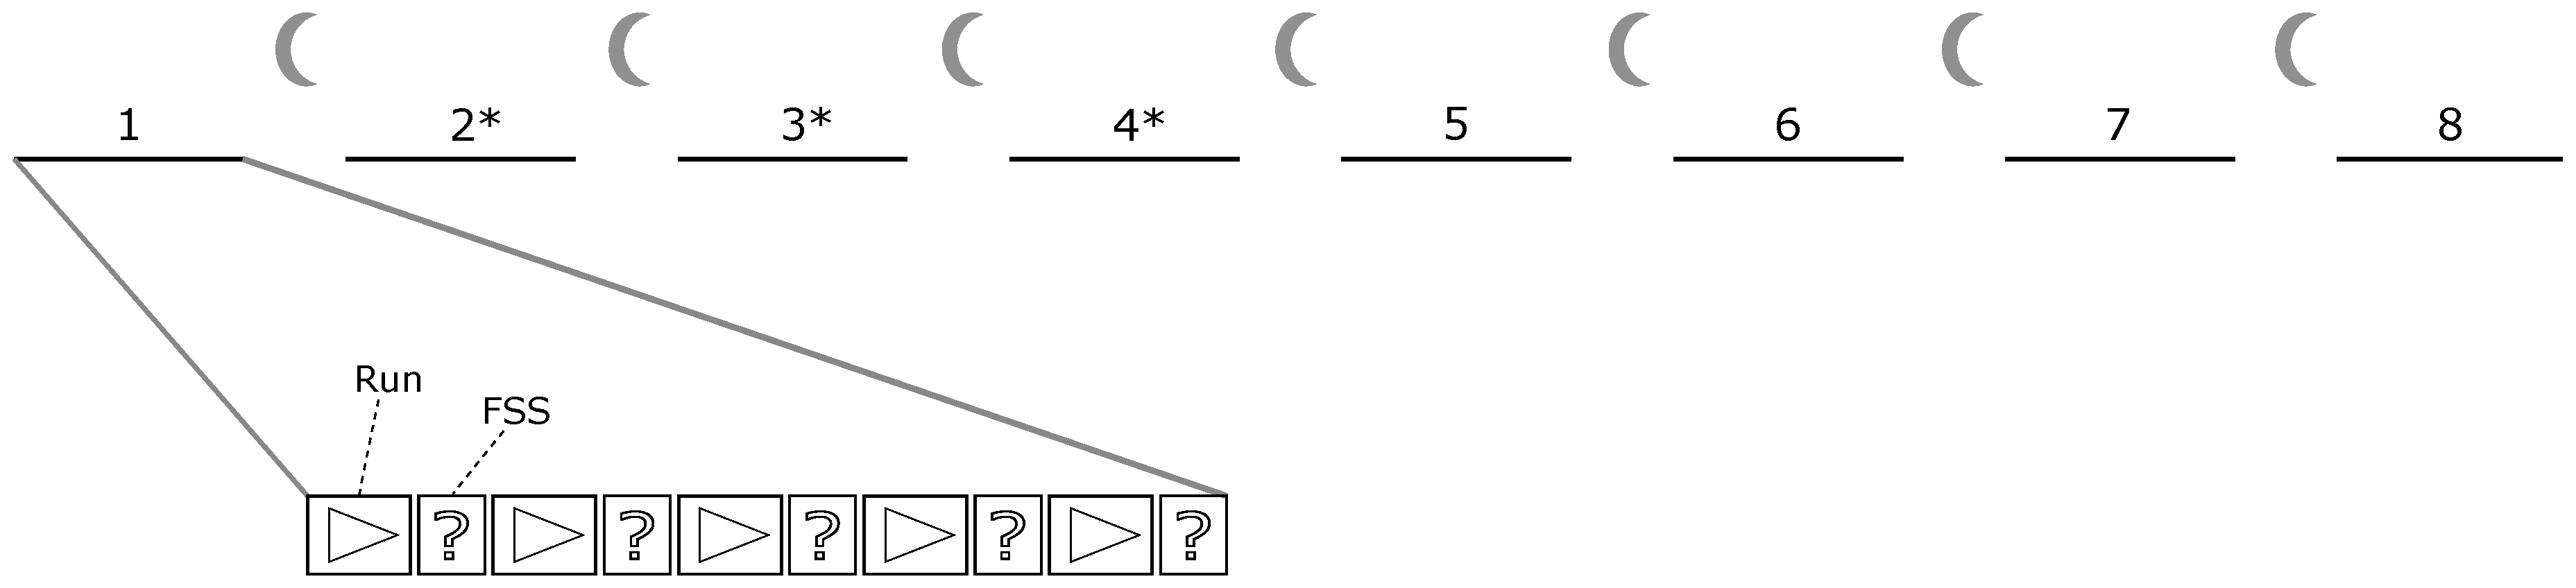
\includegraphics[width=\nicewidth]{design1}
\caption{The game was played in eight sessions on eight different days. In sessions 1 and 5--8, physiological signals were recorded during task performance; in sessions 2-4(*) no physiology was recorded. Each session consisted of five trials (2 to 4 min) followed by a self-report questionnaire (FSS, Flow Short Scale) about the latest trial.}
\label{fig:design}
\end{figure*}

\subsection*{Materials}
\paragraph{Game} The experimental task was a custom-made high-speed steering game {\it CogCarSim} designed specifically for the study of Flow and coded in Python. The game code as used herein is permanently available under open source licence at \url{https://doi.org/10.6084/m9.figshare.7269467}.

The participant steered a cube `avatar' moving forward along a straight track bounded by edges that could not be crossed. The cube's side length was 2 units, and the track was 25 units wide.  The horizontal field of view angle of the virtual camera was 60 degrees and vertical 32 degrees. The camera was positioned behind the cube at 4 units height, pointing forward along the track.

Stationary obstacles (red cones, red or yellow spheres with a height/diameter of 2 units) on the track had to be avoided. For each trial, a total of 2,000 obstacles were placed randomly on the track, with placement constrained to always allow a path through. Track length varied between 24196.4 and 24199.7 units (mean 24197.8, sd 0.8). The speed of the cube was initially set to 1.6 units per step (96 units per second); increased at a constant rate (0.0012 units/step at every step); and slowed down if obstacles were hit (0.102 units/step at each collision). When a collision caused a speed drop, the screen flashed to indicate a collision; there followed an immunity period of 100 steps during which additional collisions did not cause further speed drops. Participants could only affect speed indirectly, by avoiding collisions.  Participants were instructed to avoid as many obstacles they could in order to complete the trial as fast as possible.

The game had maximally simple one degree-of-freedom linear and holonomic dynamics: the horizontal position of the cube was directly proportional to steering wheel angle. Extensive self-piloting was done to adjust the graphics, e.g. virtual eye height; plus starting and increment speeds, rate of change of speed during collisions, and steering wheel sensitivity (steering ratio and damping).

The participants started each trial by pressing a button on the steering wheel when they felt ready. At the end of each trial, the elapsed time and number of collisions were displayed, along with a high score of the participant's ten best trials so far.

Data collected by CogCarSim included the positions, shape, and colour of obstacles on the track; trial-level aggregated performance data (trial duration, number of collisions, average velocity); and within-trial time series data (steering wheel and cube position, speed, registered collisions).

\paragraph{Equipment} The game was run on a Corsair Anne Bonny with Intel i7 7700k processor and an Nvidia GTX 1080 graphics card, running Windows 10. Eye-tracking and physiological signals were collected and stored on an Asus UX303L laptop with Debian GNU/Linux 9 OS.

The participant was seated in a Playseat Evolution Alcantara playseat (Playseats B.V., The Netherlands) aligned with the mid point of the 55" display screen (LG 55UF85). The screen resolution was 1920 x 1080 pixels, the frame rate was 60 and the refresh rate 60 Hz. The viewing distance was adjusted for each participant (so that they could place their hands on the steering wheel comfortably) and was approximately between 90 and 120 cm from the eye to the screen. The game was controlled with a Logitech G920 Driving Force steering wheel (Logitech, Fremont, CA). Steering wheel settings in Logitech Gaming Software 8.96.88 were: sensitivity 100 percent, centering spring strength 4 percent, and wheel operating range 900 degrees.

Eye movements (not reported here) were measured using Pupil Labs Binocular 120 Hz eye tracker (Pupil Labs UG haftungsbeschränkt, Berlin, Germany), stabilised with a custom-built headband. Pupil Capture software was used to collect the data from the pupil hardware. Gaze direction was calibrated using ten markers on the display, a minimum of three times during the session. Additional calibrations were done if needed. Eye movement signal was recorded at 60 Hz.

For electrodermal activity (EDA, not reported here), Ag-AgCl electrodes with 0.5\% saline paste were attached to the medial side of the left foot with adhesive skin tape and gauze. The plantar site was used instead of the palmar site to minimise artefacts resulting from the use of the steering wheel, as per guidelines by \cite{boucs12}. Blood volume pulse (BVP) was measured using a pulse oximeter sensor attached to the left index toe of each participant. EDA and BVP were recorded at 128 Hz sampling rate using NeXus-10 (Mind Media B.V, Roermond-Herten, The Netherlands) connected to a laptop via bluetooth. The data was recorded using Trusas signal acquisition software, available open access at \url{https://github.com/jampekka/trusas-nexus}.

\paragraph{Flow Short Scale} To measure self-reported Flow, participants were asked to fill in the Flow Short Scale (FSS) after each trial \citep{Rheinberg2003,Engeser2008}. FSS has 10 core items which load the subfactors {\it fluency of performance} (6 items) and {\it absorption by activity} (4 items); plus 3 items for {\it perceived importance}. The response format of FSS is a 7-point Likert scale ranging from {\it Not at all} to {\it Very much}. Higher scores on the scales indicate higher experienced Flow and perceived importance. Example items include ``My thoughts/activities run fluidly and smoothly'' ({\it fluency of performance}), ``I do not notice time passing'' ({\it absorption by activity}), and ``I must not make any mistakes here'' ({\it perceived importance}). See Supplementary Information for full English text and Finnish translation.

Cronbach's alpha for a 10-item scale including the {\it fluency of performance} and {\it absorption by activity} items was .92; Cronbach's alpha was .87 for the 13-item FSS scale including {\it perceived importance} \citep{Rheinberg2003}. FSS authors \citep{Rheinberg2003} suggest using the 10-item scale (excluding {\it perceived importance} subfactor) as a measure of experienced Flow. For our data also, Cronbach's alpha was higher for the core 10- than for 13-item scale. Thus, the Flow scale used in our analyses was formed by averaging the items in the {\it fluency of performance} and {\it absorption by activity} subfactors. The {\it perceived importance} subfactor was used separately in some analyses (see Results).

% (+3 additional items)
In addition to the 13 main items asked after every trial, participants were asked at the end of every session to report 3 more items measuring the fit of skills and demands of the task  \citep{Rheinberg2003}. These items also had 7-point scales, e.g.: ``For me personally, the current demands are... (too low -- -- just right -- -- too high)''.

There was no Finnish translation of the scale available, so it was translated into Finnish by the authors. Two of the authors (native speakers of Finnish, no formal qualifications for English-Finnish translation) first made translations independently; these translations were compared and revised, then reviewed by other Finnish-native authors, and revised.

\subsection*{Procedure}
After recruiting, participants selected eight suitable dates within a three-week period. All sessions took place between 8 a.m. and 7 p.m. at Traffic Research Unit, Department of Digital Humanities, University of Helsinki. In the first session, participants were informed about the procedure of the study and asked to fill in a background information questionnaire, including information on health, driving experience and gaming experience, and an informed consent form.

The sessions were managed by two research assistants at a time, who observed the measurement, out of participants' line of sight behind a partition wall, and took notes about possible confounding factors and problems within the session. In the beginning of each session participants filled in a session-wise questionnaire on the use of contact lenses, restedness, and medication, caffeine, and nicotine intake.

In sessions 2 to 4, participants played five trials straight after filling in the session-wise questionnaire. The FSS was filled after each trial. In sessions with physiological measurements (1 and 5 to 8), participants were dressed in physiological sensors and an eye-tracking headset, seated in the driving seat in quiet, low-light conditions for baseline measurement. They were asked to sit still for five minutes, looking at a dark blue screen, while baseline was recorded. After baseline recording, participants played five game trials, filling FSS after each trial. At the end of Session 8, the participants were debriefed and given the reward of culture vouchers.

\subsection*{Signal preprocessing and analysis}
Eye blinks were counted manually from the eye tracking videos recorded during baseline period of sessions 1 and 5--8. Three-minute periods were considered sufficient for this purpose, thus the first and last minute from each five-minute recording were omitted to obtain the most stable period of baseline. Four measurements (out of 40) were excluded due to measurement problems.

All fast and simultaneous movements of both eyelids were counted as blinks (even if the eyelid did not fully close). To ensure reliable blink identification, two of the authors independently counted the number of blinks in sessions 1, 6 and 8, and inter-rater reliability of the counts was calculated as 98.7\% (see below). We considered this high enough to have blinks in remaining sessions 5 and 7 counted by only one experimenter.

We calculated the level of consensus between the two raters as follows. Separately for each participant and session, we divide the difference of two raters' blink counts by the mean of those counts, and then subtract the quotient from 1 to obtain a percentage. All percentages are then averaged to give the overall measure of inter-rater reliability. The session-wise reliability scores also had low variability (mean of standard deviations = 0.01).

The final spontaneous eye blink rate was calculated as median blinks per minute during the
baseline measurement sessions.

\subsection*{Statistical methods}
All statistical data processing reported herein was implemented with {\sf R} platform for statistical computing \citep{R2014}. Where possible, exact corrected {\it p}-values are reported; inequalities are reported where exact values were not available. All {\it p}-values were corrected for multiple comparisons using Bonferroni-Holm. For all simple correlations we calculated Pearson's correlation coefficient, because all data in these tests were shown to be normally distributed by Shapiro-wilk tests and associated Q-Q plots. The {\sf R} code and data used to produce all analyses and figures is permanently available online at \url{https://doi.org/10.6084/m9.figshare.7268387}.
% tests   pvals    padj
% 1            LCxFlow 0.08000 0.88000
% 2           FlowXssn 0.77000 1.00000
% 3       FlowXssn1dur 0.90000 1.00000
% 4       FlowXssn2dur 0.90000 1.00000
% 5       FlowXssn3dur 0.03000 0.39000
% 6       FlowXssn4dur 0.02000 0.28000
% 7       FlowXssn5dur 0.90000 1.00000
% 8       FlowXssn6dur 0.03000 0.39000
% 9       FlowXssn7dur 0.90000 1.00000
% 10      FlowXssn8dur 0.90000 1.00000
% 11      FlowXssn9dur 0.90000 1.00000
% 12          FlowXdev 0.00020 0.00320
% 13           sEBRxLC 0.21480 1.00000
% 14         sEBRxFlow 0.70000 1.00000
% 15      FlowXsEBRdev 0.00300 0.04500
% 16  sEBRxLCxFlow+1SD 0.00001 0.00018
% 17 sEBRxLCxFlow_mean 0.00001 0.00018
% 18  sEBRxLCxFlow-1SD 0.15000 1.00000


\subsubsection*{Linear models of learning}
For {\sf RQ1}, participant-wise linear regression models were fitted using {\it lm} function in {\sf R}, which also supplies $R^2$ values. The same approach was used to fit the `grand model' to group-wise data (i.e. pooled participants).

For {\sf RQ2}, we obtained the independent variable as follows. For each participant and for each trial (40 trials in total), we subtracted predicted trial duration (y-value of power-law performance line) from observed trial duration, thus obtaining power-law model residuals, in units of log(sec). We refer to these within-participant trial-duration residuals as {\it deviation scores}, because they represent how much each observed trial duration deviates from the duration predicted by the model. Note, residuals are in the space of log-transformed trial durations in seconds and are therefore equivalent to ratio of performance in seconds. So for similar deviation scores from two trials, the later deviation represents a larger (or equal) effect in seconds.

Specifically, we first fit a linear mixed model with non-standardized Flow scores as the dependent variable, deviation scores as the predictor, and participant (numerical participant identifier ranging from 1 to 9) as a random factor with both random intercept and slope. This approach was chosen to handle the non-independence of data points within participants (see \cite{Bates2015_lme4}).

Note that that there is no consensus on the best way to obtain {\it p}-values or estimates of effect sizes from linear mixed models. We have treated the {\it t} statistic as a {\it z} statistic using a standard normal distribution as a reference, and followed the method by \cite{nakagawa2013general} to obtain pseudo-$R^2$ values. Another way to statistically evaluate the significance of these results is via the binomial distribution: The (two-tailed) probability of 9 negative slopes (should the probability of a negative slope per participant be 0.5, that is, fully random) is {\it p} = .007.
% AIC/BIC can be used to report ES for Linear mixed model if pseudo R^2 is not liked by reviewers?

\subsubsection*{Interaction analysis}
For {\sf RQ3}, to conduct a {\it simple slopes} interaction analysis we used the {\sf jtools} package for {\sf R} \citep{jtools}. The simple slopes analysis was conducted on a linear regression model (using {\it lm} function in {\sf R}) with sEBR as dependent variable; predictors were main effects of, and interaction of, Flow and LC. The slope of LC was estimated when Flow was held constant at its mean$\pm$1SD, producing the estimates shown in Table~\ref{tab:simpslopes} (see Results).


%%%%%%%%%%%%%%% END OF METHODS %%%%%%%%%%%%%%%
